\documentclass[t, aspectratio=169]{beamer}
\usepackage{amsmath,amsfonts,amsthm,amstext,amssymb, xcolor, tikz, pgf, mathrsfs, polynom, pifont, tabto}

% ----------------------------------------------------------
% Theme Setup

% Use Metropolis Theme
\usetheme[numbering=fraction]{metropolis}
\setbeamertemplate{blocks}[rounded][shadow=false]
\makeatletter
\setlength{\metropolis@titleseparator@linewidth}{1pt}
\makeatother

% Define Colors
\definecolor{chargerblue}{HTML}{002764}
\definecolor{chargerred}{HTML}{e02034}
\definecolor{bggray}{HTML}{d0d3d4}

% Set Colors
\setbeamercolor{title}{fg=chargerblue}
\setbeamercolor{background canvas}{bg=white}
\setbeamercolor{title separator}{fg=chargerred}
\setbeamercolor{structure}{fg=chargerblue}
\setbeamercolor{frametitle}{fg=white, bg=chargerblue}
\setbeamercolor*{normal text}{fg=chargerblue}
\setbeamercolor*{block body}{bg=bggray}
\setbeamercolor*{block title}{bg=chargerblue, fg=white}
% ----------------------------------------------------------

% ----------------------------------------------------------
% Custom Definitions, Commands, Environments, etc.

% Sets of numbers
\def\R{\mathbb{R}} % The reals
\def\N{\mathbb{N}} % The naturals
\def\Z{\mathbb{Z}} % The integers
\def\Q{\mathbb{Q}} % The rationals

% Blank space
\newcommand{\blank}[1]{\underline{\hspace{#1}}} % Blank space

% Change font colors
\newcommand{\cyan}[1]{{\color{cyan}{#1}}} % Changes font to cyan
\newcommand{\red}[1]{{\color{red}{#1}}} % Changes font to red
\newcommand{\magenta}[1]{{\color{magenta}{#1}}} % Changes font to magenta
\newcommand{\orange}[1]{{\color{orange}{#1}}} % Changes font to orange
\newcommand{\yellow}[1]{{\color{yellow}{#1}}} % Changes font to yellow
\newcommand{\violet}[1]{{\color{violet}{#1}}} % Changes font to violet
\newcommand{\green}[1]{{\color{green}{#1}}} % Changes font to green
\newcommand{\blue}[1]{{\color{blue}{#1}}} % Changes font to blue
\newcommand{\white}[1]{{\color{white}{#1}}} % Changes font to white

% Fitted inclusion symbols
\newcommand{\fp}[1]{\left({#1}\right)} % Fitted parentheses around content
\newcommand{\fb}[1]{\left[{#1}\right]} % Fitted brackets
\newcommand{\lhoi}[1]{\left({#1}\right]} % Left half-open interval
\newcommand{\rhoi}[1]{\left[{#1}\right)} % Right half-open interval
\newcommand{\set}[1]{\left\{{#1}\right\}} % Fitted braces (useful for sets)
\newcommand{\av}[1]{\left|{#1}\right|} % Fitted absolute value bars

% Augmented Matrix Environment
\newenvironment{amatrix}[1]{%
	\left[\begin{array}{@{}*{#1}{c}|c@{}}
	}{%
	\end{array}\right]
}

% Miscellaneous
\def\then{\Rightarrow}
\def\to{\rightarrow}
\def\d{^{\circ}}
\newcommand{\?}{\stackrel{?}{=}}
\newcommand{\cmark}{\text{ \ding{51}}}
\newcommand{\xmark}{\text{ \ding{55}}}

% Coordinate Plane (Four-Quadrant)
\def\coordplane {
	\begin{tikzpicture}        \draw[step=0.25cm,black,very thin,opacity=0.25] (-2.5cm, -2.5cm) grid (2.5cm, 2.5cm);
		\draw[<->,thick,black] (-2.5cm, 0) -- (2.5cm, 0) node[anchor=north west,pos=0.94,font=\scriptsize]{$x$};
		\draw[<->,thick,black] (0,-2.5cm) -- (0, 2.5cm) node[anchor=south east,font=\scriptsize,pos=0.94]{$y$};
	\end{tikzpicture}
}

% Coordinate Plane (One-Quadrant)
\def\onequad {
	\begin{tikzpicture}
		\draw[step=0.25cm, black, very thin, opacity=0.25] (0,0) grid (7.5cm,5cm);
		\draw[->, thick, black] (0,0) -- (7.5cm, 0) node[anchor=north west,font=\scriptsize,pos=0.94]{$x$};
		\draw[->, black, thick] (0,0) -- (0,5cm) node[anchor=south east,font=\scriptsize,pos=0.94]{$y$};
	\end{tikzpicture}
}
% ----------------------------------------------------------

% ----------------------------------------------------------
% Presentation Information
\title[3-2]{Measures of Variation}
\subtitle{Section 3-2}
\author{Jacob Ayers}
\institute{Lesson \#6}
\date{MAT 110}
% ----------------------------------------------------------

\begin{document}
	
	% Slide 1 (Title Slide)
	\begin{frame}
		\titlepage
	\end{frame}
	
	% Slide 2 (Objectives)
	\begin{frame}{Objectives}
		\begin{itemize}
			\item Find the range of a data set
			\item Find the population variance and standard deviation
			\item Find the sample variance and standard deviation
			\item Use Chebyshev's Theorem to describe data given a mean and standard deviation
			\item Use the Empirical Rule to describe data given a mean and standard deviation
		\end{itemize}
	\end{frame}

	\begin{frame}{Measures of Variation}
		In order to describe data accurately, we need to know more than the measures of central tendency.
		
		Another important aspect of a data set is its \textit{variation}, or spread. \pause
		
		There are three commonly used measures of variation: \begin{itemize}
			\item Range
			\item Variance
			\item Standard Variation
		\end{itemize} \pause
	
		We will look at each of these measures in turn; again, graphing calculators are very useful when computing them. \pause
		
		Before we start, let's look at an example to see why it is important to understand variation.
	\end{frame}

	\begin{frame}{Measures of Variation}
		A testing lab wishes to test two brands of paint to see how long each will last before fading. The lab makes 6 gallons of each brand and measures how long it lasts (in months). The data is below.
		
		\begin{tabular}{|c|c|c|c|c|c|c|} \hline
			\textbf{Brand A} & 10 & 60 & 50 & 30 & 40 & 20 \\ \hline
			\textbf{Brand B} & 35 & 45 & 30 & 35 & 40 & 25 \\ \hline
		\end{tabular} \pause
	
		If we compute the mean for each brand, we get 35 months each time (you should verify this). \pause
		
		But Brand B is significantly more consistent than Brand A is (i.e. Brand A has more variation).
	\end{frame}

	\begin{frame}{Range}
		The most basic measure of variation of variation is the \textit{range}. \pause
		
		To find the range of a data set, use the formula $R = max - min$. \pause
		
		Graphing calculators will not compute range for us, but they do report the minimum and maximum values.
	\end{frame}

	\begin{frame}{Range}
		The number of annual precipitation days  for one-half of the 50 largest U.S. cities is listed below. Find the range of the data.
		
		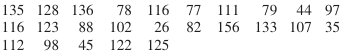
\includegraphics[width=3in]{precip-data.png} \pause
		
		By hand: $R = 156 - 26 = 130$ \pause
		
		A graphing calculator may make it easier for us to find the minimum and maximum values here.
	\end{frame}

	\begin{frame}{Variance and Standard Deviation}
		Before talking about variance and standard deviation, it's important to really understand variation. \pause
		
		Data variation is based on the distance each value is from the mean. \pause
		
		We call this difference a deviation. \pause
		
		Note: If we add all the deviations of each data value in a data set, we will always get 0. \pause
		
		To eliminate this issue, we square the deviations. \pause
		
		We then find the mean of the squares of the deviations (i.e. add them up and divide by the number of data values). \pause
		
		This average is called the variance. Since variance is given in square units, we take its square root and call this the standard deviation.
	\end{frame}

	\begin{frame}{Variance and Standard Deviation}
		Below are the formulas for the variance and standard deviation for a \textit{population}. Computing these values by hand is rather time-consuming if we don't use a graphing calculator to compute them for us. \pause
		
		Population Variance: $\sigma^2 = \dfrac{\sum (X - \mu)^2}{N}$ \\
		Population Standard Deviation: $\sigma = \sqrt{\sigma^2} = \sqrt{\dfrac{\sum (X - \mu)^2}{N}}$ \pause
		
		Note: $X$ is an individual value, $\mu$ is population mean, $N$ is population size
	\end{frame}

	\begin{frame}{Variance and Standard Deviation}
		Find the population variance and standard deviation for Brand A paint from a previous example.
		
		The data values are $10, 60, 50, 30 , 40, 20$. We computed a mean of $\mu = 35$. \pause \vspace{32pt}
		
		Using a graphing calculator, we find a population standard deviation $\sigma \approx 17.1$) (rounded). We can find the variance by squaring the standard deviation; $\sigma^2 \approx 291.7$
	\end{frame}

	\begin{frame}{Variance and Standard Deviation}
		When computing variance and standard deviation by hand, it is wise to use a table for organization. \pause
		
		\begin{tabular}{|c|c|c|} \hline
			Value $X$ & $X - \mu$ & $(X - \mu)^2$ \\ \hline
			10 & -25 & 625 \\ \hline
			60 & 25 & 625 \\ \hline
			50 & 15 & 225 \\ \hline
			30 & -5 & 25 \\ \hline
			40 & 5 & 25 \\ \hline
			20 & -15 & 225 \\ \hline
			TOTALS & 0 & 1750 \\ \hline
		\end{tabular} \pause
	
		So the variance is $\dfrac{1750}{6} \approx 291.7$ and the standard deviation is $\sqrt{\dfrac{1750}{6}} \approx 17.1$.
	\end{frame}

	\begin{frame}{Variance and Standard Deviation}
		Find the population variance and standard deviation of the precipitation data below.
		
		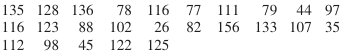
\includegraphics[width=3in]{precip-data.png} \vspace{32pt} \pause
		
		Using a graphing calculator, we find $\sigma \approx 36.1$; squaring, $\sigma \approx 1301.2$
	\end{frame}

	\begin{frame}{Variance and Standard Deviation}
		You may expect that the formula for sample variance is $\dfrac{\sum (X - \overline{X})}{n}$, but this is not the formula that is generally used. \pause
		
		The issue is that, when the population is large and the sample is small, the above formula tends to underestimate the population variance. \pause
		
		To take care of this and generate an unbiased estimator, we use the formulas below for sample variance and standard deviation. \pause
		
		Sample Variance: $s^2 = \dfrac{\sum (X - \overline{X})}{n-1}$ \\
		Sample Standard Variation: $s = \sqrt{s^2} = \sqrt{\dfrac{\sum (X - \overline{X})}{n-1}}$ \pause
		
		Note: Use the sample variance/standard deviation unless you are explicitly told to use the population values.
	\end{frame}

	\begin{frame}{Variance and Standard Deviation}
		The data show the number of public laws passed by the U.S. Congress for a sample of recent years. Find the variance and standard deviation for the data.
		
		$283, 394, 383, 580, 498, 460, 377, 482$ \pause \vspace{32pt}
		
		Using a graphing calculator, we find that $s \approx 91.5$; squaring, $s^2 \approx 8373.6$
	\end{frame}

	\begin{frame}{Variance and Standard Deviation}
		We can also find the variance and standard deviation for grouped data.
		
		This information is found the exact same way we found the mean for grouped data, if we use a graphing calculator (this is what I'll be demonstrating). \pause
		
		If you want/need to do the calculation by hand, the formulas are below.
		
		Variance: $s^2 = \dfrac{n\fp{\sum (f \cdot X_m^2)} - (\sum (f \cdot X_m))^2}{n(n-1)}$ \\
		Standard Deviation: $s = \sqrt{s^2} = \sqrt{\dfrac{n\fp{\sum (f \cdot X_m^2)} - (\sum (f \cdot X_m))^2}{n(n-1)}}$ \pause
		
		The formulas look ugly, but if we use a table to organize things, the computations are not difficult.
	\end{frame}

	\begin{frame}{Variance and Standard Deviation}
		The data show the number of murders in 25 selected cities. Find the variance and standard deviation for the data.
		
		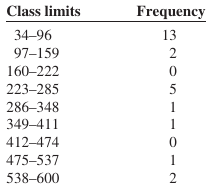
\includegraphics[width=1.5in]{murder-data.png} \pause
		
		First, find the midpoints (you should verify): $65, 128, 191, 254, 317, 380, 443, 506, 569$
		
		Now, using a graphing calculator, we find that $s \approx 167.2$. Squaring this result, $s^2 \approx 27941.8$ \pause
		
		On the next slides, I'll demonstrate solving this problem by hand. If you are using graphing calculator, you can stop watching now.
	\end{frame}

	\begin{frame}{Variance and Standard Deviation}
		\begin{tabular}{|c|c|c|c|c|c|} \hline
			Class & Midpoint & $X_m^2$ & Frequency & $f \cdot X_m$ & $f \cdot X_m^2$ \\ \hline
			34-96 & 65 & \onslide<2->{4225} & 13 & \onslide<3->{845} & \onslide<4->{54925} \\ \hline
			97-159 & 128 & \onslide<2->{16384} & 2 & \onslide<3->{256} & \onslide<4->{32768} \\ \hline
			160-222 & 191 & \onslide<2->{36481} & 0 & \onslide<3->{0} & \onslide<4->{0} \\ \hline
			223-285 & 254 & \onslide<2->{64516} & 5 & \onslide<3->{1270} & \onslide<4->{322580} \\ \hline
			286-348 & 317 & \onslide<2->{100489} & 1 & \onslide<3->{317} & \onslide<4->{100489} \\ \hline
			349-411 & 380 & \onslide<2->{144400} & 1 & \onslide<3->{380} & \onslide<4->{144400} \\ \hline
			412-474 & 443 & \onslide<2->{196249} & 0 & \onslide<3->{0} & \onslide<4->{0} \\ \hline
			475-537 & 506 & \onslide<2->{256036} & 1 & \onslide<3->{506} & \onslide<4->{256036} \\ \hline
			538-600 & 569 & \onslide<2->{323761} & 2 & \onslide<3->{1138} & \onslide<4->{647522} \\ \hline
			TOTALS &  &  & \onslide<5->{25} & \onslide<6->{4712} & \onslide<7->{1558720} \\ \hline
		\end{tabular}
	
		\onslide<8->{Now, we can use the formulas to find the variance and standard deviation.}
	\end{frame}

	\begin{frame}{Variance and Standard Deviation}
		\begin{flalign*}
			s^2 &= \dfrac{n\fp{\sum (f \cdot X_m^2)} - (\sum (f \cdot X_m))^2}{n(n-1)} & \\
			\onslide<2->{&= \dfrac{25(1558720) - (4712)^2}{25(24)}} & \\
			\onslide<3->{&= \dfrac{38968000 - 22202944}{600}} & \\
			\onslide<4->{&\approx 27941.8} & \\
			\onslide<5->{s &= \sqrt{s^2}} & \\
			\onslide<6->{&= \sqrt{27941.76}} & \\
			\onslide<7->{&\approx 167.2}
		\end{flalign*}
	\end{frame}

	\begin{frame}{Next Steps}
		\begin{itemize}
			\item Complete Assignment 3
			\item Begin Module 4 \begin{itemize}
				\item Read 3-3
				\item Watch Video Lesson \#7
			\end{itemize}
		\end{itemize}
	
		\vfill
		
		Thanks for watching!
	\end{frame}
	
\end{document}